\label{poly}
\backgroundcolor{c[1]}[HTML]{eeddff}
\backgroundcolor{C[1](0.5\columnsep,10000pt)(10000pt,10000pt)}[HTML]{eeddff}
\renewfontfamily\pagenumfont{Gentium Book Basic}[Color=222288FF] % To go with Jay
\begin{paracol}{2}
\begin{leftcolumn}

\noindent My parents put me through three divorces. My mother and father divorced when I was very young. Young to the point where I don't remember them being married. I remember finding a picture of them walking with their arms around each other's backs. Dad was shirtless and chestnut brown, hair a near-black 'fro. Mom was in a white blouse, blonde hair in a perm. It seemed so alien to me.\index{Family!mom}\index{Family!dad}

Mom and Jay got divorced when I was in my freshman year of high school. I remember being taken to a family therapy session for Jay's lingering divorce with his previous wife, but no such luck with his divorce with my mom. I just remember things getting bad after I came out, and then my mom coming downstairs to wake me one morning and inform me that we were moving out. Today. Now.

\end{leftcolumn}
\begin{rightcolumn*}
  \label{jay}
\index{Jay|(}
\renewcommand*{\footnoterule}{%
  \kern-3pt%
  \color[HTML]{222288}\hrule width 0.4\columnwidth
  \kern2.6pt}
\fontspec{Gentium Book Basic}[Color=222288FF,Ligatures=TeX]
\renewfontfamily\allyFont{Merriweather Sans}[Scale=0.9,Color=4444AAFF,Ligatures=TeX]
\noindent Mom and Jay got married when I was in elementary school. Fourth grade, maybe? It's a bit hazy.

\begin{ally}
Life began in high school, remember?
\end{ally}
Life began when I came out, I suppose. Or maybe when I ran away. Life began when I started to assert ownership over it.

\begin{ally}
Who owned it before?
\end{ally}
I thought my dad did. My dad and Jay, and they let my mom borrow me.

\begin{ally}
What did you own.
\end{ally}
Many gifts. A few hobbies. Later, an internet connection.
\newpage

\noindent Jay was a photographer. An artist. A true, honest, dyed-in-the-wool artist.

\begin{ally}
You looked up to him. Part of you wanted to be him. He could run a photography business funded by his day job of being a newspaper photographer. You thought of him when you changed your major to music.
\end{ally}
Did I? I was terrified of him.

\begin{ally}
Are they so different? `Awe', as a word, is not always a positive one.
\end{ally}
He took a picture of his son from a prior marriage that I still remember. Zach was shirtless, covered in mud that had started to dry and crack. He was looking down and to the left. He was holding something\ldots{}a sunflower, maybe? He had ram horns. The colors were muted\ldots{}was it black and white? Or was it just the mud?

I think I wanted to be that. Not Zach, necessarily. but I wanted to be that picture. I wanted to be a son that was loved like that. I wanted to be something as magical as that felt.

\begin{ally}
You also wanted to be the Phantom from Phantom of the Opera. Raoul was the bad guy, and you danced with your `Christine', Sarah Trowbridge, after school in front of your parents on the balance beam.
\end{ally}
I desperately craved being an artist. I drew endlessly. I played the saxophone, and sometimes I even liked it. I wrote music. My first song in third or fourth grade.

Maybe I did look up to him. He pulled it off.

\begin{ally}
Until he didn't.
\end{ally}
Right. When my mom told me to get in touch with him a decade and a half after the divorce, he owned a feed store down the block from me.

He left The Rocky Mountain News as lead photographer or something to pursue a job in 3D art. He bought Bryce 3D. He brought Lightwave. He spent a year learning Lightwave, and when the next version came out, he bought that and said it would take time to learn.

By that point, mom had been supporting all of us --- herself, him, me, my step-brother and two step-sisters --- for a year. She confided in me later that she had lost half a million dollars by the end of the relationship.

I didn't remember that folly. I majored in music and thought, ``Ah, yes, I can get a job doing library music or teaching choir while I work on my compositions'' but forgot how lucky he was when I met him.

\begin{ally}
You remembered and raced to teach yourself programming.
\end{ally}
\emph{You} remembered, maybe. I'd like to think of myself as a bit of a dreamer, even still.

\begin{ally}
Thus you, 1:19 AM on a Tuesday, gritting your teeth and trying not to write about mania.
\end{ally}
\newpage

\noindent Our punishment --- my step-siblings and I --- was time-out. Jay had an old church pew rescued from some church in New Mexico that he'd painted a grayish sky blue. ``Go sit on the bench,'' he'd tell us. ``Half an hour.''

\begin{ally}
You measured it with your fingers. You'd judge the width of the plank you sat on by pinching it. Three inches? Four? You'd lay your length on it and count how many Matts it took from one end to another.
\end{ally}
It was a perfect punishment. My dad lamented once that he couldn't send me to my room as a punishment because I'd happily sit in there for hours on end.

\begin{ally}
You'd be away from him. That's a reward.
\end{ally}
I hadn't thought of it that way.

The bench, though, was perfect. It faced a dining table,\footnote{\color[HTML]{222288}A dream: \emph{I am moving through the house, and suddenly a flood of brightly colored scorpions starts to pile in through the doors and windows. They're bright and plastic like Creepy Crawlers, but I know they'll be deadly. I have to hide under the dining room table. There is a flash, and then I'm riding on the table like a raft, but I have to be careful, as it is as if it's on a fulcrum and if I row or punt too hard, it will flip over, burying me in scorpions.}}\index{Dream} and across from that, the computer which was kept powered off. No reading. No talking. No moving from the bench. If more than one of us were in trouble at the same time, no looking at each other; we sat on opposite ends.

When he started taking up martial arts, he brought Zach and I with him. He thought\ldots{}well, I don't know what he thought. That it would make us men? That it would teach us to defend ourselves?

In the end, it turned into its own means of punishment. He'd grapple with us. He'd grab me by the front of my shirt and slam me into the cabinets. It was just play, right? Just studying up for the next session, right?

\begin{ally}
Maybe he wanted to hit you from the start. Maybe that's why he got into karate.
\end{ally}
I think part of him did, yeah. I think part of him would rather our punishments would make him feel better at the same time. It took me a while to think of it that way, though. It took me a while to think of it as abuse.

\begin{ally}
It took you no longer being afraid of him. It took you telling your mom that, no, you wouldn't go see him at his feed store in Loveland. It took you until then to think of it as anything other than you not being man enough.
\end{ally}
I'm still afraid of him. Maybe it just took me admitting that.
\newpage

\noindent When I came out, I did so by leaving a book of stories from gay youth on top of my mom's reading pile right before taking the bus down to visit my dad for the night. She called me after dinner and asked me if the book meant what she thought it did.

\begin{ally}
Did you ever tell --- really tell, with words and everything --- any of your family you were gay? Or trans?
\end{ally}
Twice. It was awful.

She must have told him at some point. Within a week, he told my mom I had to tell Zach that I was gay, too. He left the house on a run and made my mom stand in the kitchen with me to make me say, ``Zach, I'm gay.''

He just said, ``Oh, okay'', and kept pouring his Kix.

\begin{ally}
And then he stopped talking to you.
\end{ally}
Beside the point.

After I came out, Jay changed. He got mean--

\begin{ally}
``Got'', she says.
\end{ally}
Do you fear him, then?

\begin{ally}
Mu.
\end{ally}
Fair enough.

He got mean. That's when he got physical. That's when his anger got hot.

He started reading my emails. He found some reply notifications to some posts on a forum, where kids were talking about puberty. As kids do, there was some dick-size comparing. He read that aloud in front of my mom and mocked me for my answer. I had said seven inches. It was generous, sure, but keep in mind, I was way underweight at the time--

\begin{ally}
And him rather overweight.
\end{ally}
--and the skinnier you are, the less padding you have around the base of your penis.

\begin{ally}
We're getting off topic.
\end{ally}
Are we? I was starting to own my body. I was starting to find things that I felt I could feel proud about. I was starting to form relationships. Puberty was in full swing and I was realizing that there were people my age like me who would find me attractive.

And he took that and he humiliated me for it.

\begin{ally}
Let's talk about kink.
\end{ally}
Let's fucking not.
\newpage

\noindent My mom and I got in the habit of going to the dog part after work. We'd pick up Hank, our golden lad, and Chelsea, our Phyllis-Diller-slash-Yoda mutt, and drive across town to a field dedicated to letting dogs frolic with each other.

We'd play with other dogs. We'd through tennis ball after slobbery tennis ball. We got to know the other owners, mostly as ``oh, you're Sandy's owner''.

\begin{ally}
Or ``oh, you're Zephyr's owner''. You stole your own dog's name from some random aussie shepherd at the dog park.
\end{ally}
It was a meaningful period of my life. Is there some reason that wouldn't make a big impact on me?

\begin{ally}
It was Zephyr or Samuel. Even you knew what you wanted. You had him already named in your mind.
\end{ally}
And mom and I would talk. We'd walk the perimeter or, on hot days, sit at the lone picnic table under the lone tree and talk.

I was sitting on the table itself, feet on the bench, and she was sitting next to me, when she said, ``I think I'm going to get divorced from Jay. Is it alright if I use his reaction to you coming out as the reason?''

\begin{ally}
And you thought, ``I must be the luckiest boy in the world, being able to say that I knew my parents' divorce was your fault.''
\end{ally}
She told me how much money she had lost, and how he had changed even before I came out. I think that's when I realized that she might be a friend as well as a mother.

\begin{ally}
Gag.
\end{ally}
I know. I tried typing that eight different ways, and no matter what, it sounds like a Care Bears thing or whatever.

\begin{ally}
Back to the lilac-scented word, please.
\end{ally}
Gladly.
\newpage

\noindent Between when the divorce was decided and when we were supposed to move out to the townhouse my mom had purchased, mom adopted a dog. Helen had clearly been feral rather than a surrender, because she was impossible. She didn't know how to act around dogs. She didn't know how to act around people. She didn't know how to act indoors. She didn't know how to act outside.

\begin{ally}
She didn't know how to act around you, so you hid from her.
\end{ally}
She didn't know how to act around Jay, either, to be fair. One night, three days before we were supposed to move out, mom was sleeping on the couch downstairs, and Jay came down from the master bedroom to have the last word in one argument or another, and Helen raced up to greet him, nailing him right in the nuts with her paw.

Do you laugh?

\begin{ally}
Not my department.
\end{ally}
It took my mom and I a while to laugh about that. It's the type of story that usually gets a laugh, right? Nut-shots?

\begin{ally}
Hollywood decrees it must be so.
\end{ally}
Maybe my mom smiled when she woke me to tell me we had to move out immediately. It was Sunday. We moved all we could to the townhouse in my mom's Honda Civic and slept on newly-purchased air mattresses. Mine kept going flat.

\begin{ally}
Your mom would soon learn that she had rheumatoid arthritis. You complained to her about that in the morning, and she stayed quiet about how much pain she must have been in.
\end{ally}
The next day at school was nigh intolerable.

\begin{ally}
And yet you felt free.
\end{ally}
And yet I felt free.
\newpage
\renewcommand*{\footnoterule}{\oldfootnoterule}
\index{Jay|)}

\end{rightcolumn*}
\begin{leftcolumn}

I don't remember ever seeing Jay again after that, though I surely must have.

\begin{ally}
But you heard about him.
\end{ally}
Mom said he called Erin, my ex-step-sister a ``witch''. I don't think that's the word he used. A decade and a half later, she'd suggest that I go visit him.

I turned her down.

\begin{ally}
A sub-story. Do I sense conflict?
\end{ally}
Of course.

\begin{ally}
You may be made of star-stuff, but conflict seems to be what holds you together.
\end{ally}
Stop trying to get me to talk about mania.

At first, I was proud of my relationships. Then I was embarrassed. There were so many, all in a line. One would trickle into existence with, as I put it, \emph{light, in through the head, out through the heart}. We'd be perfect, until we weren't. Everything would be delightful, until it wasn't. It's the way of early relationships, I suppose. You fall for someone, and you can't quite pick apart the difference between love and lust.

I just went through so many that I started feeling a bit weird about it. How do I talk about the Danny-Marek-Merlin-Andrew-Michael-Andy-Rikky-Kayla-Tyson-Andrew(again) progression? And how do I talk about Lon? Or what JD and I were at the beginning?

\begin{ally}
Doubtless with the same lilac-scented words you talk about everything.
\end{ally}
I guess.

Early on, I promised myself that I would do anything to not become my dad, in so many ways. One of those was to not run my relationships like him. Some bits were easy, of course. I could start by being queer. That's glib, of course, but at the time I started dating, being queer required more discretion, more discussion than I saw in my dad's relationships.

Some bits weren't so easy, though. The overlap between the discussion that's involved the mechanics of simply having a queer relationship and the discussion that's involved in having a healthy relationship, queer or not, is not non-existent, but neither is it large.

\begin{ally}
Are you going to provide us with a Venn Diagram? In hand-coded SVG, perhaps?
\end{ally}


\noindent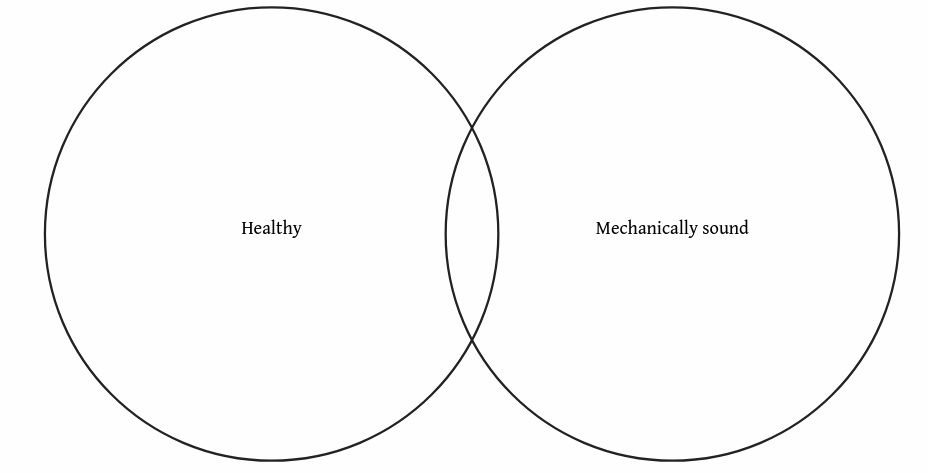
\includegraphics[width=4.25in]{assets/static/healthy-sound.png}

Happy?

\begin{ally}
Very. I just wanted to ensure that you were at your very Maddy-est about this.\index{Catastrophically Maddy}
\end{ally}
When my dad divorced Julie, he told her he hadn't loved her in ten years. He told her he married her because she was easy to deal with. Quiet. Compliant. Not as smart as him. He could be right around her, which wasn't always guaranteed with mom.

Julie's friends gave her a rubber rat afterward. They had scribbled his name on it. The rat was sitting on a plaque that said \texttt{Rat\ Bastard}. The last time I saw her, she was very drunk, sagged against my side, sobbing and beating that rat against the nightstand.\index{Family!Julie}

\begin{ally}
And you didn't want to be like him when you grew up? Color me surprised.
\end{ally}
You \emph{would} say that.

He had started dating well before divorcing her. I don't know if he and Maurine are married now. When I told mom, she shrugged and said that he had started dating Julie before their own divorce.

\begin{ally}
You dovetailed relationships. You were dating Andrew well before you and Tyson fell away from each other.
\end{ally}
Hey, I said some bits weren't as easy. He left me with a lot of him in me.

\begin{ally}
Like the anger. He gave you that. The anger and the pride.
\end{ally}
I pay for his past as well as mine.

So, when Michael mentioned that he wanted to go on a date with someone else while we were together, well, it touched a nerve.
\newpage

\begin{ally}
I suppose you also searched your archives for poly.
\end{ally}
You know me so well.

\begin{ally}
Of course.
\end{ally}
The first mention on LiveJournal was April 6th, 2004.

\index{Journal entries}
\begin{quotation}
Of the interesting topics that popped up, that of polygamy stuck with me the most.  Michael\index{Relationships!Michael} has a date with another on Thursday and, while this brought up issues with Merlin and Atrius, all I can say right now to Michael is that I wish him the best of luck.  It just feels like it would actually /work/ in his case.  As to how it pertains to me, I'm not sure if my mind could handle having two mates.  Granted I still have a thing for Kory (hah, good luck with that) and a few others, I just don't think I could find another who a) would be willing to have that sort of relationship with me and b) I could have that sort of relationship with.  Ah well.  Something to think about.
\end{quotation}

\begin{ally}
Never one to have a high opinion of yourself.
\end{ally}
That's hindsight talking.

\begin{ally}
You literally just got out of a therapy session where you talked about how you don't believe you deserve a better job.
\end{ally}
Touché.

Michael and I's relationship was rocky, tumultuous. We met through a queer group and from there wound up in a weird, heated romance that danced around sex, gender, mental health, everything. We fought, we made up. We got annoying. We made out a lot, we had sex, though with each of our individual hangups around sex, it was rarely penetrative.

\begin{ally}
It was penetrative once.
\end{ally}
That's rare, isn't it?

\begin{ally}
Vanishingly.
\end{ally}
Listen, we were both trans. The subject was complex.\index{Gender}

\begin{ally}
You were a cis gay guy. You told me that. You were unsure of vaginas.
\end{ally}
It started that way, I suppose. I learned.

\begin{ally}
Then you bought one for yourself.
\end{ally}
Listen.

\begin{ally}
Yes?
\end{ally}
There were bits of sexuality that didn't work for me when I was bepenised. A lot of those make sense in a transgender context. Matthew was still a gay guy, but the Ship-of-Theseusizing was already beginning.\index{The Death of Matthew}\index{Ship of Theseus}

\begin{ally}
`Bepenised'? `Ship-of-Theseusizing'?
\end{ally}
You verbed it first.

\begin{ally}
We've gotten off track.\index{ally}
\end{ally}
Right.

In two previous relationships, poly had come up, and neither time, it had worked. With Merlin and Atrius, I had immediately jumped to jealousy. I felt as though I was being set aside.\index{Relationships!Merlin}

\begin{ally}
Never one to have a high opinion of yourself.
\end{ally}
It didn't last. That was part of the breaking point. Similarly with Andrew and Ryn. I've heard it said that jealousy is a sign that one's needs are not being met.

\begin{ally}
What did you need that you weren't getting?
\end{ally}
I thought it was someone to myself.

\begin{ally}
You couldn't own yourself, maybe you could own someone else.
\end{ally}
That hurts to hear.

\begin{ally}
Is it wrong?
\end{ally}
I don't know. Maybe it isn't. Maybe I wanted to keep someone. To possess them. Maybe it was a reaction to being owned.

\begin{ally}
Let's talk about kink.
\end{ally}
Let's fucking not.
\newpage

\noindent I won't repost them, because they're direct logs, shortly after the conversation mentioned before, the issue of Michael bringing another partner to the queer group we were a part of came up. How would we work a situation where I, coming from a monogamous point of view, would be in the same room with my partner and metamour? Would we split our time? Would one of us get ignored while the other got attention? Would we both get attention? Would we just plain avoid it?

\begin{ally}
It's surreal, even for me, to hear you talk about this today, given your current situation.
\end{ally}
Suppose that the young man, Matthew, is in a monogamous relationship with someone. As the years go by the relationship begins to change, fades, and is replaced by a new one, more open than the last. After a decade or so, all of the parts have been replaced and Matthew, now Madison, is in a polycule the size of Rhode Island. Is Madison still the same person as Matthew?

\begin{ally}
That's a bit heavy-handed.
\end{ally}
You can't start the metaphor train a-rollin' and then expect it to stop on a dime.

\begin{ally}
I'll own that.
\end{ally}
I met JD in 2005, and met Robin in 2012. By 2013, I was in a relationship with both, and we were sharing dinner, along with Robin's partner, at a convention. It was natural. Comfortable. It was fun.

And now, I'm in relationships of various sorts with a half dozen people. The changes between then were so incremental, and discussed so thoroughly, that it really does feel Ship of Theseish.\index{Ship of Theseus}

\begin{ally}
Stop.
\end{ally}
Never.

The other consequence of that is that, along the way, I sufficiently distanced myself from the mechanics of my parents' relationships that I finally felt comfortable in calling that dream fulfilled. The turning point was my mom, during one of her visits back to Colorado, mentioned my relationship with Robin as something she could never do.

\begin{ally}
Are you sure it wasn't writing a Python/Javascript/SVG web app to map polycules using force-directed layouts?\index{Catastrophically Maddy}
\end{ally}
Okay, maybe it was before then.

\begin{ally}
And score a point to the ally.
\end{ally}
I didn't feel better than my mom when she said that, of course. Her relationships matured well over time, I think. She and Bob got better at communicating and expressing their needs. And even if they hadn't, the love she had for all of her partners was no less valid for being monogamous.

\begin{ally}
Could you say the same of your dad, had he said that to you?
\end{ally}
I don't know.

\begin{ally}
Probably not.
\end{ally}
Yeah, probably not.
\newpage

\noindent Relationship anarchy, as a topic, seems to draw heavily from both poly folks and queer folks. In fact, the three ideas are so heavily intertwined that it's difficult to have one without the others. Poly? Well, there's a good chance that there are some queer aspects to your relationship.

And if you're queer and at least of a certain age, relationship anarchy is baked into your soul. If your society sets up a ``natural'' relationship progression and then bars an entire class from entry to that progression, subversive and transgressive relationship structures form as a matter of course.

\begin{ally}
Queer people, queer relationships.
\end{ally}
Yes. June, 2004:\index{Journal entries}

\begin{quotation}
Queer hair, queer mouth, queer brain, queer sleeves, queer shoes, queer toes, queer nails, queer fingers, queer palms, hairy palms, queer wrists, limp wrists, queer arms, queer shoulders, arms around shoulders, queer neck, sensitive neck, queer hair, curly, queer ears, sensitive ears, eargasmic, queer cheek, blushing cheek, queer nose, got it from my dad, queer eyes, queer colors, got them from my grandpa, queer eyebrows, but not as queer as some, queer face, too long, queer chest, too skinny, queer belly, padded, queer crotch, go figure, queer thighs, better believe it, queer knees, queer calfs, queer ankles, queer legs, flexible, queer feet, still smell, queer guy, no surprise.
\end{quotation}

\noindent When you're queer, \emph{being queer} is baked into just about everything about you, but most especially in your relationships. ``Minority identity acts as a force multiplier on social dynamics,'' as Orrery put it.

\begin{ally}
And so?
\end{ally}
And so, being hopelessly queer, I wind up in relationships that are hopelessly queer.

\begin{ally}
Except when you don't.
\end{ally}
Yes. And when I don't, there's such a fundamental mismatch of understanding that I feel uncomfortable in my own skin.

Something that queer relationships miss, or at least reconfigure to their own ends, is the relationship escalator, that heteronormative idea that one gets on at the ground floor of friendship and gets off at the top with marriage, or one can stop off at any of the other floors to stop for a while, or to step off entirely when the relationship ends.

It's not a bad idea, either. It's not as old as some would have you think, but in today's society, it works quite well.

\begin{ally}
Does the divorce rate agree with you there?
\end{ally}
Is that just another step on the escalator?

\begin{ally}
Touché.
\end{ally}
In nonheteronormaitve relationships, the idea is muddied. The friends-dating-marriage-children set of steps, originally shattered whe marriage was made illegal and adoption banned for large swaths of queer folks, just doesn't fit. The barrier between friends and dating, as well as between dating and permanent relationship, is thin, osmotic.

\begin{ally}
Suddenly, you're in a relationship. Suddenly, you're saying ``I love you.''
\end{ally}
Yes. Suddenly, organically, though not for lack of deliberation. There's much talking, if everything goes right, much working out of boundaries. It's just that there are fewer milestones.

\begin{ally}
Why do you bring this up? You're not writing an article. Out with it.
\end{ally}
Right.
\newpage

\noindent If poly is queer, in that it's not relationship-normative, then I'm queer. If being trans is queer because it's not gender-normative, then I'm queer. If my identity blurs lines, then I'm queer.

If I'm in a relationship with someone, then, is that a queer relationship? Is my partner queer?

\begin{ally}
What would they say?
\end{ally}
I don't know. I haven't gotten to the point of talking to myself about this yet, much less talking with them. That's what this process is, isn't it?

\begin{ally}
So what would you say, then?
\end{ally}
My gut instinct says that, since I'm trans, I've transgressed the lines of gender-normative relationships; since I'm poly, I've transgressed the lines of relationship-normative relationships. That, since I am queer, the relationship must be as well.\index{Gender}

\begin{ally}
But?
\end{ally}
But it doesn't really feel like it. I feel like a girlfriend. Barac feels like a boyfriend. I feel like I've stepped onto an escalator, here.

\begin{ally}
There is an error in your gut instinct: it does not take into account that, in a relationship between two people, there are more than just two actors. There is you, there is your past, there is Barac and his, and there is society, influencing all four of you. That you are queer and that Barac does not consider himself to be is beside the point. Society, Barac, and Barac's past all think of this as a straight relationship --- or a take on one, at least --- and that's overwhelming your gut instinct, which only has access to you, and limited access to your past.
\end{ally}
Is that why I feel contention, then? Is that why there are an odd number of actors in this situation?

\begin{ally}
Perhaps. Perhaps you are feeling contention because you are having to work, for once, rather than slot smoothly into a relationship.
\end{ally}
My other relationships have taken work, though.

\begin{ally}
Your other partners have spoken the same language as you. It was easier to coordinate that work. You and Barac are having to learn each other's language as you go along.\index{Relationships!Barac}
\end{ally}
Robin and I had to learn the language of poly when we were starting out together. Judith and I and Colton and I both had our own things to learn as our relationships grew. Justin and I had to figure out our boundaries together.\index{Relationships!Judith}\index{Relationships!Colton}\index{Relationships!Justin}

\begin{ally}
Yes, but you all spoke queer. None of you really spoke normative, a skill you're having to learn late in life.
\end{ally}
\newpage

\noindent I've been married for eight years. Robin and I have been together for more than six. I've been with both Judith and Justin for more than five. My polycule has grown steadily over the years, and I have to wonder: how much of my polyamory, my relationship anarchy is a coping mechanism for how I was raised?\index{Relationships!JD}\index{Relationships!Robin}\index{Relationships!Judith}\index{Relationships!Justin}

\begin{ally}
Does it matter?
\end{ally}
Yes, I think it does. \emph{Early on, I promised myself that I would do anything to not become my dad,} I said. I wanted to stay away from serial monogamy. I wanted to talk more and perform less within my relationships. I wanted to be an improvement upon what I saw growing up.

If I'm poly because I'm coping for my past once again, have I really grown? Or have I fallen into the trap just on the other side of the path?

If I'm coping for my childhood, what would I leave my children coping with?

\begin{ally}
Again, does it matter? You must walk a fine line between the selfish and selfless when working with reality. In order to be happy, you need to not repeat the past, as you've said --- a selfish act. But worrying about counterfactuals with non-existent entities, being \textbf{too} selfless in this, will only set you back in your own growth.
\end{ally}
Perhaps I'm worried that if poly and such are just coping mechanisms, my relationships might be somehow less real, less earnest than if they weren't. Perhaps I'm worried that I'm doing a disservice to my partners by using them to overcome my own failings.

\begin{ally}
This is impostor syndrome, not using people. No relationship is perfect, all that matters is that you're approaching these honestly, earnestly, and with your whole heart. Even then, there will be friction occasionally. Your parents gave you stuff to cope with, and you would give your children stuff to cope with too.
\end{ally}
Guess it's a good thing I don't have kids.

\begin{ally}
Let's talk about kink.
\end{ally}
Oh my \emph{god}.

\begin{ally}
Alas, had I a face, I would be able to smirk. Imagine that for me, will you?
\end{ally}
You know what? Now's as good a time as any.
\newpage

\end{leftcolumn}
\end{paracol}
\resetbackgroundcolor

\renewfontfamily\pagenumfont{Gentium Book Basic}[Color=000000FF]
\index{Relationships!polyamory|)}
